\par Dans cette partie nous allons ainsi vous présenter les trois briques logicielles réalisé pour ce projet et les méthodes de pré-traitement réalisés :

\begin{itemize}
	\item Pré-traitement : formatage des données
	\item Détermination du sentiment du tweet
	\item Détermination de l'opinion towards
	\item 
\end{itemize}

\section{Chargement des données}

Lors de l'étude des données, ne nous sommes rendu compte que le jeu de données d'apprentissage et de test ne comportent pas le même nombre de ". En effet, les tweets concernant le sujet "Donald Trump" ont été ajouté dans le jeu de test.

N'étant pas dans les conditions réelles de la compétition, nous avons décidé de fusionner l'ensemble des datasets afin de les redécouper de manière aléatoire en trois ensembles, l'un d'apprentissage, l'un de test pour tester les différents modèles, et l'un de "validation" \textbf{utilisé une seule fois} dans notre projet pour la prédiction.


\section{Formatage des données}
\par Afin d'améliorer les performances des différents blocs de cette implémentation, nous avons choisi de formater au mieux les données. Uniquement les tweets sont concernés pas ce formatage.

\par Plusieurs méthodes ont été appliquées:
\begin{itemize}
  \item transformation en minuscule de tous les caractères en majuscule.
  \item suppression du hashag \#semst présent à la fin de chaque tweet, et n'apportant aucun caractère informatif au tweets.
  \item remplacement des symboles pouvant être exprimés par des mots en ledit mot. Par exemple, au symbole \% correspond le mot "percent", au symbole \& le mot "and", ...
  \item suppression de tous les symboles ne pouvant pas être exprimés pas des mots, en particulier les symboles de ponctuation.
  \item transformation des formes contractées en leur forme étendue. Par exemple, à "ma'am" correspond le mot "madam", à "I'm" les mots "I am".
  \item transformation des nombres en le mot "number". En effet, la valeur exprimée n'a pas d'influence sur le sens du tweet.
  \item transformation des mentions (utilisation du symbole @) d'utilisateurs, en le mot "someone". Dans certains contextes, la valeur de cette mention pourrait être intéressante (dans le cas ou on arriverait à déterminer si cette mention a une valeur positive ou non par exemple), mais de part l'implémentation que nous avons choisi, ce formatage est plus pertinent, et améliore l'apprentissage du bloc "Opinion towards" detection.
  \item transformation de tous les verbes en leur forme infinitive.
\end{itemize}

\par Quelques autres formatages des tweets pourraient être pertinents dans le cadre de ce projet:
\begin{itemize}
  \item si plusieurs mots ont un synonyme en commun, il pourrait s'avérer judicieux de remplacer lesdits mots par ce synonyme. Ainsi, nous réduisons le dictionnaire de mots utilisés, et pouvons améliorer l'apprentissage du bloc "Opinion towards" detection.
  \item il est compliqué d'extraire le sens des hashags utilisés dans les tweets, cependant il correspondent régulièrement à un groupe de mots collés. Ainsi un hashag comme \#NetNeutrality pourrait être décomposé en deux mots, "net" et "neutrality".
  \item transformation des mots au pluriel en leur forme au singulier. En effet, ils seront interprétés comme étant des mots différents par le bloc "Opinion towards" detection, alors qu'ils n'influent pas sur sens général du tweet.
  \item suppression des répétitions de mots.
\end{itemize}
Certains formatage appliqués ne sont pas forcément des plus précis, et pourraient être améliorés. Par exemple, dans le cas du remplacement des contractions en mots, il est difficile de déterminer si "he's" correspond à "he is" ou "he has".

\section{Sentiment analysis}

\par Concernant la partie détection de sentiment l'objectif est de déterminer si le tweet est "positif", "neutre" ou "négatif". 
\par Pour déterminer la méthode la plus efficace nous avons réaliser une comparaison de plusieurs méthodes :

\begin{itemize}
	\item Étude du sentiment des Tweets à l'aide de la polarité positive, négative et neutre de chaque mot des Tweets via l'utilisation de Sentiwordnet.
	\item Étude du sentiment des Tweets à l'aide de la polarité positive, négative et neutre de chaque mot des Tweets via l'utilisation de Sentiwordnet et de Wordnet.
	\item Détermination du sentiment des Tweets à l'aide de classifier.
\end{itemize}

\subsection{Sentiwordnet}
\par Sentiwordnet est un dictionnaire de mots de référence avec lequel on va travailler dans cette partie.
\par Sentiwordnet permet d'obtenir des scores entre 0 et 1 informant de la forte positivité ou de la forte négativité d'un mot donné. \\


\par \textbf{Principe :} \\
\par Prendre une liste de tweets en entrée. Pour chacun des tweets on va sommer les scores de positivité ainsi que les scores de négativité de tous les mots du tweets. Pour obtenir le score de polarité final du tweet on va soustraire le score de négativité au score de positivité. \\

\par \textbf{Étape de la méthode :} \\
\begin{itemize}
	\item Pré-traitement : Retrait des mots de liaison, déterminant, ponctuation, symbole qui n'ont pas d'impact dans la détermination de la polarité des mots.	 \\
	\item Part Of Speech Tagging : Utilisation de la librairie nltk (Natural Language Toolkit) afin de tagger chaque mots des tweets par leur description grammatical tel que NN pour "nom" ou JJ pour "adjectif". Le but de faire ça dans cette méthode et de pouvoir filtrer les catégories de mots que l'on va donner en entrée de Sentiwordnet pour déterminer leur polarité dans le but d'avoir un meilleur résultat en étudiant les catégories les plus pertinentes. Nous avons donc choisi d'étudier les scores de positivité et de négativité des groupes NN (noms), JJ (adjectifs), VB (verbe), RB (adverbe). \\
	\item Calcul du sentiments de tous les mots retenus dans un tweet pour obtenir la polarité moyenne du tweet. \\
	\item Si le score final du tweet est positif alors la prédiction du tweet est 'positif', si le score est négatif on retourne 'négatif' et si le score vaut 0 on retourne 'neutre'. \\
\end{itemize}

\par \textbf{Résultats :} \\

\begin{table}[h!]
\centering
\caption{Résultats Sentiwordnet}
\label{my-label}
\begin{tabular}{|l|l|}
\hline
                   & Taux de bonne prédiction \\ \hline
Sans-prétraitement & 48,9\%                   \\ \hline
Avec-prétraitement & 54,6\%                   \\ \hline
\end{tabular}
\end{table}



\subsection{Wordnet}

\par L'objectif dans cette méthode est d'utiliser un autre dictionnaire pour étudier la polarité des mots des tweets car le dictionnaire Sentiwordnet possède un lexique restreint ne permettant pas de calculer la polarité de tous les mots donc beaucoup ne sont pas étudié. \\

\par L'avantage avec Wordnet c'est que l'on va extraire les mots des tweets et pour tous les mots on va à l'aide de Wordnet récupérer le mot le plus général du mot en entrée. Par exemple grâce à sa reconnaissance de synonyme wordnet va transformer les mots "sorrowful" et "sad" par le mot "unhappy". Ainsi l'avantage ici c'est que l'on va appliquer la même méthode que précédemment avec Sentiwornet pour le calcul de polarité mais grâce à l'utilisation de Wordnet en amont le dictionnaire Sentiwornet pourra calculer le score de davantage de mots car les mots non présent dans ce dictionnaire auront été remplacé par des mots plus basiques bien présent dans Sentiwornet. \\ 

\par Dans la méthode précédente on a pu constater que les pré-traitement étaient utiles donc nous les avons conserver dans cette méthode également. \\

\par\textbf{ Résultats : } 53,19\%

\subsection{Classifiers}

\par Dans cette partie nous allons nous concentrer sur de la prédiction de sentiment à l'aide de classifier. Contrairement aux deux autres partie nous allons avoir besoin de deux jeux de données, un jeu de donnée d'apprentissage et un jeu de donnée de test. Ainsi à partir du jeu d'apprentissage on va construire notre modèle de prédiction et on va prédire sur les données de test. \\

\par Pour l'utilisation de classifier nous nous sommes tourné vers l'utilisation de la librairie scikit-learn et nltk. \\

\par \textbf{Principe : } \\
\par Pour l'apprentissage les classifier nltk fonctionne avec des structures de caractéristiques, dans notre cas avec des dictionnaires associant le nom d'une caractéristique à une valeur. 
\par D'après une étude bibliographique nous nous sommes tourné vers l'étude de Naive Bayes Classifier dans un premier temps puis ensuite sur des classifiers alternatif.  
\par Nous utilisons ce type de classifier basées sur les fréquences de mots associées à chaque étiquette de positif ou négatif. \\

\par Sur le jeu d'apprentissage pour construire le modèle on va utiliser les informations suivantes : \\
\begin{itemize}
	\item Tweet\_train
	\item Sentiment\_train \\
\end{itemize}


\par \textbf{Étape de la méthode :} \\
\begin{itemize}
	\item Étape 1 : Création des dictionnaires de caractéristiques. On va récupérer trois listes contenant tous les tweets dont le sentiment est 'positif', 'négatif' ou 'neutre' et pour chacune des listes on va créer trois nouvelles listes contenant tous les mots relatif à un tweet positive, négatif ou neutre. Pour optimiser l'analyse qui va suivre on ne conservera que les mots de plus de 6 caractères. A partir de l'extraction des mots de chaque labels, on va construire les dictionnaires de caractéristiques nécessaire à l'utilisation des classifiers. \\
	\item Étape 2 : Avec l'utilisation des librairies on va pouvoir construire des classifiers et estimer la précision des classifiers. On va apprendre le modèle sur un set d'apprentissage composait des structures de caractéristiques pour label positif, négatif et neutre d'apprentissage et on va calculer la précision du modèle avec les structures de caractéristiques de test pour label positif, négatif et neutre du jeu de test. \\
\end{itemize}

\par \textbf{Méthode alternative }: \\
\par Dans la méthode décrite précédemment on construisait nous même nos dictionnaires de caractéristiques mais il est possible d'utiliser les outils de librairies pour les remplacer comme la méthode TF*IDF comme méthode de pondération pour obtenir les structures de caractéristiques pour mettre en place les classifier.
\par C'est donc avec la méthode TF*IDF que nous avons également construit nos classifier et que nous avons évaluer le taux de bonne prédictions.

\par \textbf{Résultats :} \\


\begin{table}[h!]
\centering
\caption{Comparaison des taux de bonne prédiction des classifiers selon deux méthodes}
\label{my-label}
\begin{tabular}{|l|l|l|}
\hline
                   & \begin{tabular}[c]{@{}l@{}}Précision des classifiers avec \\ des dictionnaires de caractéristiques manuel\end{tabular} & \begin{tabular}[c]{@{}l@{}}Taux de bonne prédiction\\ avec la méthode TF*IDS\end{tabular} \\ \hline
BernoulliNB        & 66.9\%                                                                                                                 & 71.2\%                                                                                    \\ \hline
MultinomialNB      & 67.1\%                                                                                                                 & 69,2\%                                                                                    \\ \hline
LogisticRegression & 66.8\%                                                                                                                 & 72.7\%                                                                                    \\ \hline
SGDClassifier      & 63,3\%                                                                                                                 & 70,9\%                                                                                    \\ \hline
SVC                & 65\%                                                                                                                   & 65\%                                                                                      \\ \hline
LinearSVC          & 61,6\%                                                                                                                 & 72.1\%                                                                                    \\ \hline
\end{tabular}
\end{table}

\par \textbf{Conclusion :} \\
\par La méthode la plus efficace est la méthode utilisant TD*IDF avec le classifier Regression Logistique. \\


 
\section{"Opinion towards" detection}

\section{Stance detection}

La partie "Stance detection" consiste à déterminer l'opinion du tweet par rapport au sujet, c'est-à-dire si le tweet est "pour", "contre" ou "neutre" vis à vis du sujet. Cette étape prend en entrée le "Target" (le sujet), le "Sentiment" (positif, négatif ou autre) et l'"Opinion Towards" (le tweet donne un opinion par rapport au sujet, le tweet donne un opinion qui n'a pas de rapport avec le sujet, ou le tweet ne donne pas d'opinion). Ces deux derniers sont déterminés dans les étapes précédentes. Cette dernière étape est donc sensible aux taux d'erreur précédemment obtenus.
La combinaison de ces trois entrées permet de déterminer la "stance". \\

Cette partie est un problème de classification basique, qui prend en entrée trois paramètres qui renvoie une sortie. C'est un problème de classification multi-classe, en effet la sortie se compose de 3 classes : "FAVOR", "AGAINST" et "NONE". \\

\subsection{POC - Traitement des données}

Une première approche a été de tester différentes méthodes de classification usuelles comme SVM et bayes.

Pour cela, un petit traitement sur les données s'impose, effectivement pour utiliser de telles méthodes il est d'abord nécessaire de labelliser les données avec des classes numérotées pour s'abstraire des chaînes de caractères. \\
Dans le jeu de données de train fourni, il y 5 "target" différents, en ce qui concerne le "sentiment" il y a 3 classes possibles et il en est de même pour l'"opinion towards".

En essayant de réaliser une SVM, nous nous sommes rendu compte que dans le jeu de données de test il y avait maintenant 6 "target". En effet, les tweets concernant le sujet "Donald Trump" ont été ajouté. Or, le modèle ne peut pas fonctionner pour un sujet qui n'a pas été appris. 
La solution a dont été de fusionner les ensembles d'apprentissage et de test et de les redécouper de manière aléatoire afin d'obtenir des tweets de l'ensemble des "target" dans l'ensemble d'apprentissage.

\subsection{POC - Test de méthodes de classification}

Tout d'abord, nous avions décidé d'implémenter une méthode de classification bayésienne et une méthode SVM, ensuite il a également été possible d'implémenter d'autres méthodes classification.

Pour un premier test, toutes les méthodes ont été testées avec les paramètres par défaut, et renvoient les taux d'erreurs suivants :
\begin{itemize}
\item Bayes avec un noyau Gaussien : 31,74$\%$
\item SVM Linéaire : 37,62$\%$
\item SVM : 33,11$\%$
\item K plus proches voisins : 34,47$\%$
%\item Arbre de décision : 24,49$\%$
\end{itemize}

Les résultats de ce POC sont disponibles dans la section \hyperref[annexe-stance-detection]{Annexe : POC - Find Stance} p.2-3.

\subsection{POC - Test de paramètres de la méthode SVM}

Ensuite, il s'est avéré intéressant de tester différents paramètres de la méthode SVM. Le résultat est présent sur la figure suivante.

\begin{figure}[!h]
\centering
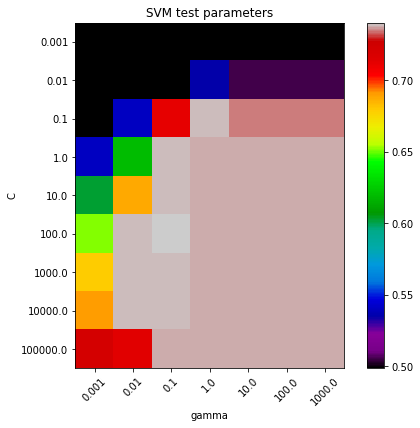
\includegraphics{src/annexes/POC_FindStance_V2/output_24_0.png}
\end{figure}

\textbf{Les valeurs C=100 et gamma=0.1 ont donc été choisi pour réaliser cette SVM, qui fournit finalement un taux d'erreur de $24,49\%$}.

C'est donc cette méthode qui a été implémentée
\subsection{Implémentation d'une SVM}




